%
% Quantum Algorithms
%

\section{Quantum algorithms} \index{Quantum algorithms}\label{sec:quantum_algs}

The ultimate goal of quantum computing is to implement algorithms with a quantum speedup compared to classical algorithms. The degree of speedup achieved varies between algorithms, and it is important to note that not every classical algorithm exhibits any speedup when implemented quantum mechanically.

To provide context for the excitement of quantum computing and motivate interest in their development, we now summarise some of the key quantum algorithms that have been described exhibiting quantum speedup.

%
% Deutsch-Jozsa
%

\subsection{Deutsch-Jozsa} \index{Deutsch-Jozsa algorithm}

The first quantum algorithm demonstrating a provable improvement over the best classical algorithm was the Deutsch-Jozsa algorithm\cite{bib:DeutschJozsa92}. Unfortunately the algorithm solves a very contrived problem, designed for the purposes of demonstrating post-classicality rather than solving a problem of actual practical interest. Nonetheless, the algorithm is straightforward to explain and understand, making it a useful starting point in understanding quantum algorithms and the computational enhancement they may offer.

The algorithm relies on a `black box', referred to as an \textit{oracle}\index{Oracle}, which takes an input bit-string and outputs a single bit, evaluating the function $f(x)$ for the $n$-bit input bit-string $x$. In this contrived problem $f(x)$ is guaranteed to be either \textit{uniform}\index{Uniform function} or \textit{balanced}\index{Balanced function}. In the former case, the output to the oracle is always \mbox{$f(x)=0$} or always \mbox{$f(x)=1$}, but it doesn't matter which, they simply must always be the same. In the latter case, the output is \mbox{$f(x)=0$} for exactly half the inputs $x$, and \mbox{$f(x)=1$} for the other half of $x$, but the ordering of which inputs generate which outputs may be arbitrary. The goal of the algorithm is to determine whether $f(x)$ is uniform of balanced using the least number of queries to the oracle.

While it's clear that the dimensionality of the input state space is exponentially large, $2^n$, it is fairly obvious that a trivial \textbf{BPP} algorithm exists for solving this problem with confidence exponentially asymptoting to unity against the number of oracle queries. We simply evaluate the oracle for randomly chosen inputs. If we measure any occurrences of measurement outcomes that are not all 0 or all 1 we know with certainty that the function must have been balanced. If on the other hand we measure all 0s or all 1s for more than half the input state space $x$, we know with certainty the function was uniform.

However, if the function were balanced, there is the possibility that it might conspire against us to fool us into thinking the function was uniform until we evaluate half plus one of the input states, requiring $O(2^n)$ oracle queries, although this will occur with exponentially low probability against the number of queries. Thus, the algorithm can be approximated with exponential asymptotic certainty in \textbf{BPP}\index{\textbf{BPP}}. But considering the \textit{worst} case\index{Worst case complexity} rather than the \textit{average} case\index{Average case complexity}, we may have to perform an exponential number of evaluations, $O(2^n)$, to know the answer with absolute certainty.

The Deutsch-Jozsa algorithm solves this rather specialised problem in the worst case using only a single quantum evaluation of the oracle.

The algorithm implementing the Deutsch-Jozsa protocol and its circuit diagram are shown in Alg.~\ref{alg:deutsch_jozsa}. The engine room of the algorithm is in the Hadamard transform\index{Hadamard transform}, $\hat{H}^{\otimes n}$, which prepares an equal superposition of all $2^n$ possible input bit-strings $x$, which are then evaluated in superposition by the oracle. To ensure unitarity, the oracle is defined to implement the transformation\footnote{Note that the seemingly more obvious choice of \mbox{$\hat{U}_f\ket{x}=\ket{f(x)}$} is not unitary. This trick of introducing an additional ancillary state to enable unitary construction of arbitrary functions is a common one in quantum algorithm design.},
\begin{align}
	    \hat{U}_f \ket{x}\ket{y} &= \ket{x}\ket{y\oplus f(x)}.
\end{align}
That is, it flips bit $y$ if \mbox{$f(x)=1$} (equivalently addition modulo 2 or an XOR operation). An inverse Hadamard transform subsequently yields a measurement outcome with one of two possibilities:
\begin{itemize}
	\item The 0 and 1 terms outputted from the oracle interfere perfectly constructively, if the function was uniform.
	\item They interfere perfectly destructively, if the function was balanced.
\end{itemize}
Then, with a single-shot measurement of the inverse Hadamard transformed output from the oracle we establish whether $f(x)$ was balanced or uniform with certainty. This exhibits an exponential worst case speedup compared to a randomised classical sampling algorithm (which is classically optimal).

\begin{table}[!htb]
\fbox{\parbox{0.965\columnwidth}{\texttt{ 
function DeutschJozsa(f,n):
\begin{enumerate}
    \item Prepare the \mbox{$n+1$}-bit state,
    \begin{align}
    \ket\psi_0 = \ket{0}^{\otimes n}\ket{1}.	
    \end{align}
    \item Apply the \mbox{$n+1$}-bit Hadamard transform across all qubits,
    \begin{align}
    \ket\psi_1 &= \hat{H}^{\otimes(n+1)}\ket\psi_0 \nonumber \\
    &= \frac{1}{\sqrt{2^{n+1}}} \sum_{x=0}^{2^n-1}\ket{x}(\ket{0}-\ket{1}),	
    \end{align}
    where $x$ denote $n$-bit binary bit-strings, of which there are $2^n$.
    \item Apply the unitary oracle, implementing the transformation,
    \begin{align}
    \hat{U}_f \ket{x}\ket{y} &= \ket{x}\ket{y\oplus f(x)},
    \end{align}
    where $\oplus$ denotes addition modulo 2, yielding,
    \begin{align}
    \ket\psi_2 = \hat{U}_f \ket\psi_1.	
    \end{align}
    \item Apply another Hadamard transform,
    \begin{align}
    \ket\psi_3 = \hat{H}^{\otimes n} \ket\psi_2.
    \end{align}
    \item The full evolution is thus given by,
    \begin{align}
    	\ket\psi_\text{out} = (\hat{H}^{\otimes n}\otimes\hat{I}) \cdot \hat{U}_f \cdot \hat{H}^{\otimes (n+1)}\ket{0}^{\otimes n}\ket{1}.
    \end{align}
	\item Measure the first $n$ qubits to determine the probability of measurement outcome $\ket{0}^{\otimes n}$.
	\item This probability is given by,
	\begin{align}
	P_0 = \left| \frac{1}{2^n} \sum_{x=0}^{2^n-1} (-1)^{f(x)} \right|^2.	
	\end{align}
	\item Depending on whether $f(x)$ was uniform or balanced, the alternating sign terms in this sum interfere constructively or destructively, yielding \mbox{$P_0=1$} or \mbox{$P_0=0$} respectively.
	\item Thus, a single measurement outcome suffices to determine whether $f(x)$ was balanced or uniform.
	\item $\Box$
\end{enumerate}
\begin{align}
\Qcircuit @C=1em @R=1.6em {
    \lstick{\ket{0}^{\otimes n}} & \gate{\hat{H}^{\otimes n}} & \multigate{1}{\hat{U}_f} & \gate{\hat{H}^{\otimes n}} & \meter \\
    \lstick{\ket{1}} & \gate{\hat{H}} & \ghost{\hat{U}_f} & \qw & \\
} \nonumber
\end{align}
}}}
\caption{Deutsch-Jozsa algorithm for evaluating whether the function $f(x)$ implemented by the oracle is balanced or uniform, exhibiting exponential worst case speedup compared to the best classical \textbf{BPP} algorithm.} \label{alg:deutsch_jozsa}
\end{table}

%
% Quantum Search
%

\subsection{Quantum search} \index{Grover's algorithm}

The problem of finding specific entries in unstructured data spaces is a ubiquitous one. This class of \textit{search algorithms} have amongst the broadest applicability of any class of algorithms. Computer scientists have invested excruciating man-hours\index{SJW}\footnote{Presently, most computer science research institutions are equal opportunity employers.} into organising and structuring data so as to minimise the resource overhead (in time and/or space) associated with extracting desired components. However, the methodology for achieving this, and the favourability of associated resource overheads, is highly dependent on the structure of the underlying data, or whether there even is any. To this end, numerous data structures and algorithms have been developed, accommodating for every mutation and variation of the posed problem imaginable. Often, there is a tradeoff between the overheads induced in time and memory, as well as in pre-processing and data structure maintenance requirements.

For example, \textit{hash tables}\index{Hash tables} enable theoretical $O(1)$ lookup times on data with a \textit{key-value pair}\index{Key-value pair} data structure. In a key-value pair each data entry (value) is tagged with a unique identifier (key) used for lookup. The value can observe any structure whatsoever, whereas the key is designed so as to minimise search times. When storing telephone numbers one might represent entries as key-value pairs, where the keys are people's names, and the values their respective telephone numbers. An efficient algorithm for mapping keys to physical memory addresses would imply efficient lookup of telephone numbers by name.

In the absence of a key-value representation one might simply store data in sorted form. However, this requires pre-sorting the entire data space, which may become costly for large data sets, and requires continual rearrangement whenever the data space is modified, making it computationally costly for mutable datasets.

For the end user, who wishes to find data elements, the worst-case data space is one with no order or underlying structure. Suppose we want to find whether a number exists in the telephone directory, but we don't know it's associated name. In this instance, it can easily be seen that the best one can hope for, in terms of algorithmic runtime, is to simply look through the data space brute-force\index{Brute-force} until we find what we are looking for. It is clear that with an unstructured space of $N$ elements, this brute-force search algorithm requires on average $O(N)$ queries to find the desired entry. We call this the \textit{unstructured search problem}.

The brute-force classical algorithm, despite already being technically `efficient' (i.e $O(N)$ linear runtime), could nonetheless become unwieldy for very large datasets. Google doesn't want to exhaustively scan their entire collection of data-centres each time they want to lookup a database element. The quantum search algorithm, first presented by Grover \cite{grover1997quantum}, provides a solution to this problem using only $O(\sqrt{N})$ runtime (oracle queries), a quadratic enhancement. Whilst this falls far short of the exponential quantum enhancement one might have hoped for, which has also shown to be optimal \cite{bennett1997strengths, zalka1999grover}, it is nonetheless still extremely helpful for many purposes, given the broad applications for this algorithm.

We will formulate the quantum search algorithm as an oracular algorithm\index{Oracle}, where the oracle takes as input an $n$-bit string, and outputs 1 if the input matches the entry we are looking for, otherwise 0. This formulation of the problem makes the algorithm naturally suited to solving satisfiability problems (many of which are \textbf{NP}-complete and of great practical interest).

The Grover quantum search algorithm is shown explicitly in Alg.~\ref{alg:quant_search}.

\begin{table}[!htb]
\fbox{\parbox{0.965\columnwidth}{\texttt{ 
function Grover(f,n):
\begin{enumerate}
	\item Using a Hadamard transform, prepare the $n$-qubit equal superposition of all $2^n$ logical basis states,
    \begin{align}
    \ket\varphi &= \hat{H}^{\otimes n}\ket{0}^{\otimes n}	 \nonumber \\
    &= \frac{1}{\sqrt{2^n}}\sum_{x = 0}^{2^n - 1}\ket{x},
    \end{align}
    where $x$ denotes a bit-string of length $n$.
	\item The oracle is defined as a unitary black-box, which tags a target element $T$ using a phase-flip,
	\begin{align}
		\hat{U}_T \ket{x} &= (-1)^{f(x)}\ket{x} \nonumber \\
		&= (\hat{I} - 2\ket{T}\bra{T})\ket{x},
	\end{align}
	where $f(x)=\{0,1\}$ is the black-box function determining whether input $x$ is the target element $T$ (\mbox{$f(x)=1$}) or not (\mbox{$f(x)=0$}).
	\item The Grover diffusion operator\index{Grover diffusion operator} is defined to implement,
	\begin{align}
	\hat{U}_s = \hat{I} - 2\ket{T}\bra{T}.
	\end{align}
    \item repeat $O(N)$ times:
    \setlength{\itemindent}{.2in}
    \item $\ket{\varphi_{i+1}} = \hat{U}_s\cdot\hat{U}_T\ket{\varphi_i}$.
    \setlength{\itemindent}{0in}
    \item $\Box$
    \item \comment{What about measurement stage}
\end{enumerate}
}}}
\caption{.} \label{alg:quant_search}
\end{table}

%
% Phase-Estimation
%

\subsection{Phase-estimation}\index{Phase-estimation algorithm}\label{sec:phasea_est_alg}

\comment{To do}

%
% Optimisation, Satisfiability & NP-Complete Problems
%

\subsection{Optimisation, satisfiability \& \textbf{NP}-complete problems}\index{Optimisation problems}\index{\textbf{NP}-complete problems}\index{Satisfiability problems}

Many readers will have heard of the \textit{travelling salesman problem}\index{Travelling salesman problem}, the task of finding the shortest route through a weighted graph that traverses every vertex. This task is known to be \textbf{NP}-complete.

Many other algorithms are also known to be \textbf{NP}-complete, a number of which that are relevant to networking are discussed in detail in Sec.~\ref{sec:graph_theory}, summarised in Table.~\ref{tab:net_alg_sum}.

Such \textbf{NP}-complete algorithms can be quadratically enhanced in runtime using Grover's algorithm. To see this, note that all \textbf{NP}-complete problems can be efficiently mapped to one another with polynomial resource overhead (see Fig.~\ref{fig:complexity_classes}). Thus, we can restrict ourselves to considering the satisfiability problems\index{Satisfiability problems} discussed above -- the archetypal \textbf{NP}-complete problems. An example of the {\sc 3-SAT} problem\index{3-\textsc{SAT} problem }, which is \textbf{NP}-complete, is shown in Fig.~\ref{fig:3SAT}.

\begin{figure}[!htb]
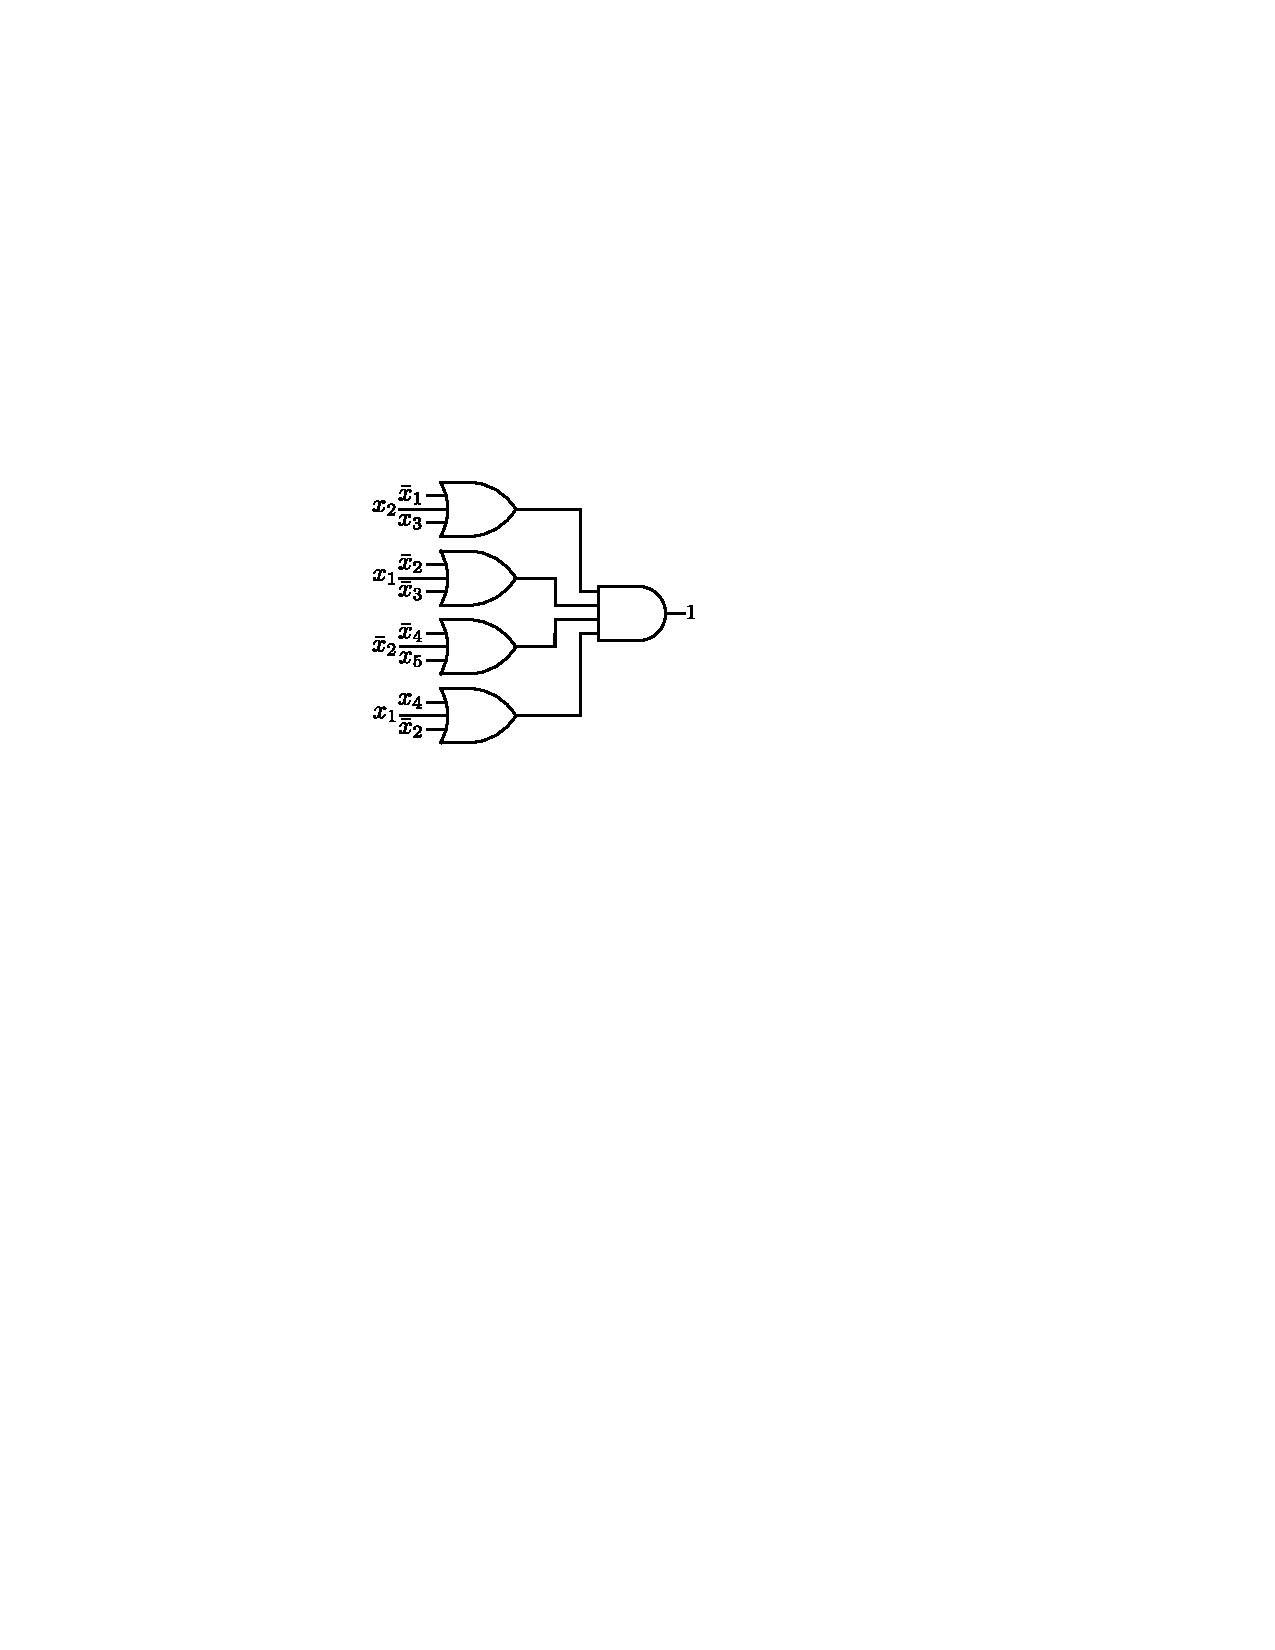
\includegraphics[width=0.3\textwidth]{3SAT}
\caption{Digital circuit for an instance of the {\sc 3-SAT} problem. Each or the OR gates is input with some combination of the input bits or their compliments (i.e with a NOT gate). Each of these is referred to as a `clause', of which there are 4 in this example, but could be any number in general. The final AND gate requires that all clauses be simultaneously satisfied in order to yield a final output of `1'. The goal of the problem is to find an input bit-string that yields an output of `1'. In general, this may require exhaustively searching over the entire space of input states via brute-force, which exhibits time-complexity exponential in the length of the bit-string. This problem is proven to be \textbf{NP}-complete.} \label{fig:3SAT}	
\end{figure}

Now, by defining an oracle that implements a polynomial-time algorithm on $n$ qubits, a Grover search over the input space of $2^n$ configurations will determine the satisfying input to the oracle for a given desired output, which acts as the tagged element within the search algorithm. The Grover search yields a quadratic speedup for this search compared to a brute-force classical search, therefore requiring only $O(2^{n/2})$ oracle calls. While this is short of the exponential speedup one might hope for, a quadratic speedup can nonetheless be very significant for large instances of the problems.

Some problems in even harder classes than \textbf{NP}-complete can in some instances be \textit{approximated} using the same approach. The key to solving such problems is to define an oracle that attributes a \textit{score} to a given input, rather than a yes/no answer to satisfiability, and answers `yes' or `no' depending on whether that score is above some defined threshold. As an illustrative example, consider the optimisation of, say, a complex traffic network, where the goal is to maximise flow through the network. Then we might define our score to be some flow metric for the network's graph.

We then apply a Grover search repeatedly, each time incrementing this threshold until the algorithm outputs `no'. Then we know that the last input had the highest score. The reason this approach is \textit{approximate} rather than \textit{exact} is that defining such a score-oracle mightn't be always efficiently implemented, or maybe it mightn't make sense at all to define score measures for a given problem.

%
% Quantum Simulation
%

\subsection{Quantum simulation} \index{Quantum chemistry}\index{Quantum simulation}\index{Hamiltonian simulation}\label{sec:quantum_sim_alg}

\comment{To do - Zuen}

\cite{bib:lloyd1996universal}

\comment{Discuss quantum chemistry as leading application}

%
% Integer Factorisation
%

\subsection{Integer factorisation} \index{Shor's algorithm}\index{Hidden subgroup problem}\index{Period-finding algorithm}\index{Discrete logarithm algorithm}

\comment{To do - Heliang}

\comment{Mention relationship to hidden subgroup, period-finding, and discrete-log problems}

While this algorithm is known to reside in \textbf{BQP}, it is strongly believed not to be \textbf{BQP}-complete. Similarly, while it is known to reside in \textbf{NP}, it is strongly believed not to be \textbf{NP}-complete, thereby placing it in the `limbo zone' of \textbf{NP}-intermediate complexity.\index{\textbf{NP}-intermediate}

%
% Quantum Machine Learning
%

\subsection{Quantum machine learning} \index{Quantum machine learning}

\cite{bib:lloyd2013quantum}

\comment{To do - Chris}

%
% Topological Data Analysis
%

\subsection{Topological data analysis} \index{Topological data analysis}

The internet currently comprises extraordinary amounts of data, from which useful information must be extracted if this vast amount of data is to be utilised effectively. For example, firms like Google and Facebook must extract meaningful information from their databases of user behaviour in order to make appropriate advertising suggestions. This task is extremely valuable -- a small improvement in a recommendation engine\index{Recommendation engine}, for example, could be worth many millions of dollars in revenue.

Performing analyses like these extremely computationally challenging when dealing with such enormous datasets as Facebook's user database or Google's website database, so-called \textit{big data analysis}\index{Big data analysis}.

One avenue for the analysis of large, complex datasets is via homology theory\index{Homology theory}, which yields \textit{topological data analysis} (TDA)\index{Topological data analysis}. In particular, the so-called \textit{Betti numbers}\index{Betti numbers} characterise the nature of interconnectedness within a dataset. Specifically, the $k$ Betti number, $\beta_k$, is the number of $k$-dimensional holes and voids in a dataset. For example, $\beta_0$, $\beta_1$ and $\beta_2$ represents the number of connected components, 1-dimensional holes, and 2-dimensional voids in a dataset respectively.

Calculating Betti numbers exactly is known to be \textbf{PSPACE}-complete\index{\textbf{PSPACE}-complete}\footnote{\textbf{PSPACE} is the complexity class of problems requiring polynomial memory with unbounded runtime, a class that is not classically efficient.}, and the best-known classical approximation algorithm has runtime,
\begin{align}
O(2^n \mathrm{log}(1/\delta)),
\end{align}
for accuracy $\delta$.

Recently, improved quantum algorithms for approximating the Betti numbers have been presented \cite{bib:lloyd2016quantum, bib:PhysRevLett.113.130503, bib:GiovannettiLloyd08}, with runtime of only,
\begin{align}
O(n^5/\delta).
\end{align}
An elementary experimental demonstration of this algorithm has been performed using a small dataset \cite{bib:LuRohdeTDAopt}.

Taking a dataset with well-defined distances between data-points (where `distance' could be any arbitrary metric in any dimension), we begin by applying a distance cutoff $\epsilon$\index{Distance cutoff} to define connections between data-points. We define $k$-simplices\index{Simplex} within the dataset, which are fully connected subsets of \mbox{$k+1$} data-points, with \mbox{$k(k+1)/2$} edges. The full set of simplices defines the dataset's \textit{simplicial complex}\index{Simplicial complex} for a given distance cutoff $\epsilon$. Construction of the so-called Vietoris-Rips simplicial complex is described in Fig.~\ref{fig:TDA_simplex}.

\begin{figure}[!htb]
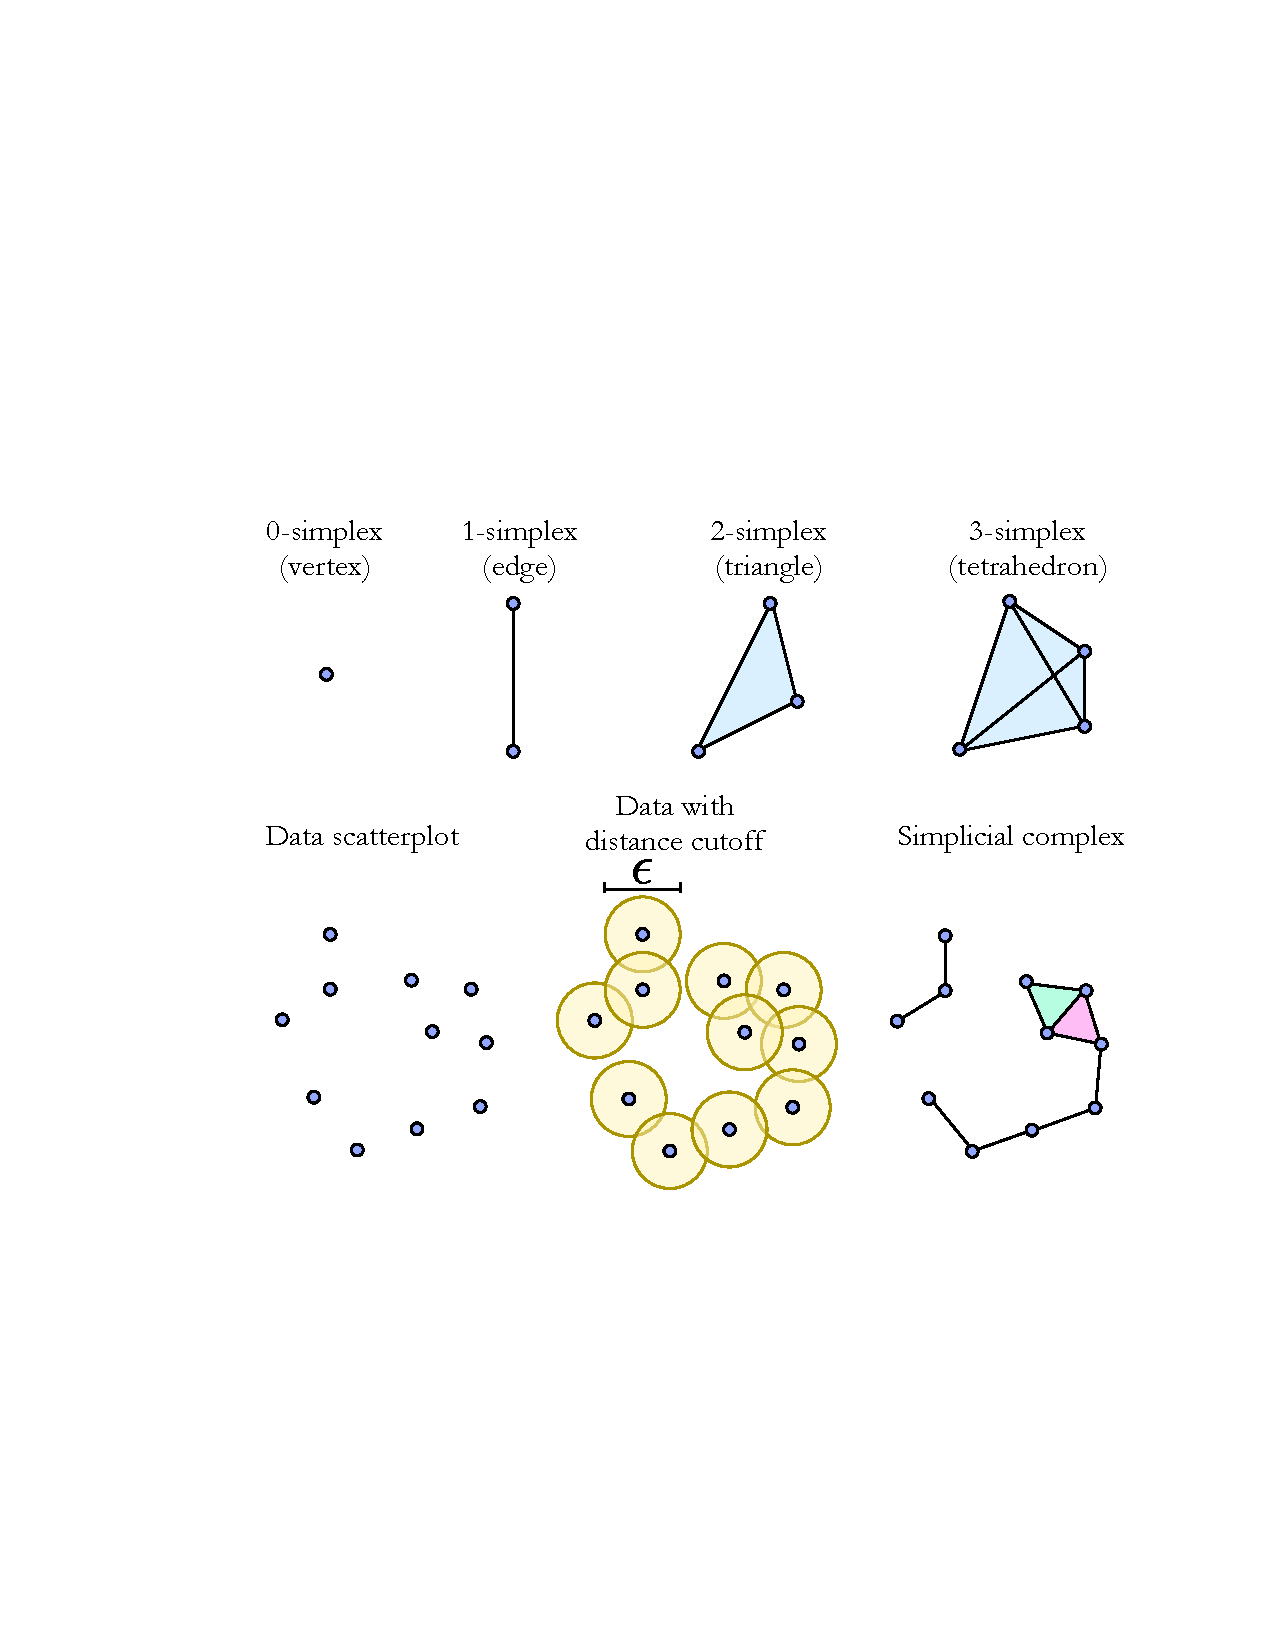
\includegraphics[width=0.47\textwidth]{TDA}
\caption{(top) Simplices\index{Simplex} are constructed as fully connected subgraphs of the data of different dimensions. (bottom) A distance cutoff is applied to create edges within a scatterplot of raw data, from which the simplicial complex\index{Simplicial complex} is constructed.} \label{fig:TDA_simplex}	
\end{figure}

The first step in the algorithm is to construct the simplicial complex superposition state,
\begin{align}
\ket\psi_k^\epsilon = \frac{1}{\sqrt{|S_k^\epsilon|}} \sum_{s_k\in S_k^\epsilon} \ket{s_k},
\end{align}
where $s_k$ denotes a $k$-simplex from the simplicial complex $S_k^\epsilon$. This superposition can be constructed by employing a Grover search using a set-membership oracle function\index{Oracle},
\begin{align}
f_\epsilon(s_k) = \left\{ \begin{matrix}
 1, & \text{if}\,\,s_k\in S_k^\epsilon, \\
 0, & \text{otherwise,}
\end{matrix}\right.
\end{align}
yielding quadratically enhanced efficiency in the simplicial complex state preparation.

From the superposition state, the mixed state,
\begin{align}
\hat\rho_k^\epsilon = \frac{1}{|S_k^\epsilon|} \sum_{s_k\in S_k^\epsilon} \ket{s_k}\bra{s_k},
\end{align}
is easily prepared with the addition of CNOT gates and ancillary qubits.

The quantum TDA algorithm then takes the simplicial complex mixed state and estimates the full set of Betti numbers by employing a phase-estimation algorithm\index{Phase-estimation algorithm} (Sec.~\ref{sec:phasea_est_alg}), which induces an exponential algorithmic runtime improvement.

Performing the TDA across a range of $\epsilon$ yields a \textit{barcode}\index{Barcode} representation for the dataset's topology. Topological features which persist over large ranges of $\epsilon$ can then be regarded as robust features of the dataset, whereas ones which only persist over a small range of $\epsilon$ can be regarded as localised, non-persistent features, which might correspond to noise for example, and be filtered out prior to further analysis. The barcode representation thereby gives us an extremely robust characterisation of the topology of the data in a scale-dependent way.

As an example for how this type of technique might be applied, consider Facebook's user database. The distance metric might relate to how similar users' interests are, or how closely related they are via their friendship networks. Then examining the barcode representation of the data by scanning over $\epsilon$ would provide insight into the persistence and robustness of these relationships at different scales within the network. At different scales we could investigate topological relationships and features at the level of individuals, family or friendship networks, communities, common interest groups, between cities, or nationally, for example.

%
% Linear Systems
%

\subsection{Linear systems} \index{Linear systems}

\cite{bib:harrow2009quantum}

\comment{To do}

\comment{Example: recommendation algorithm where sampling the vector yields, with high probability, a recommendation that is a good one, without having to explicitly know the entire solution vector.}

%
% Intermediate Models for Quantum Computation
%

\subsection{Intermediate models for quantum computation}

\comment{To do}

\index{Galton board}
\index{Sampling problems}

Sec.~\ref{sec:BS}
\comment{Boson-sampling and IQP. Other sampling problems.}

\begin{figure}[!htb]
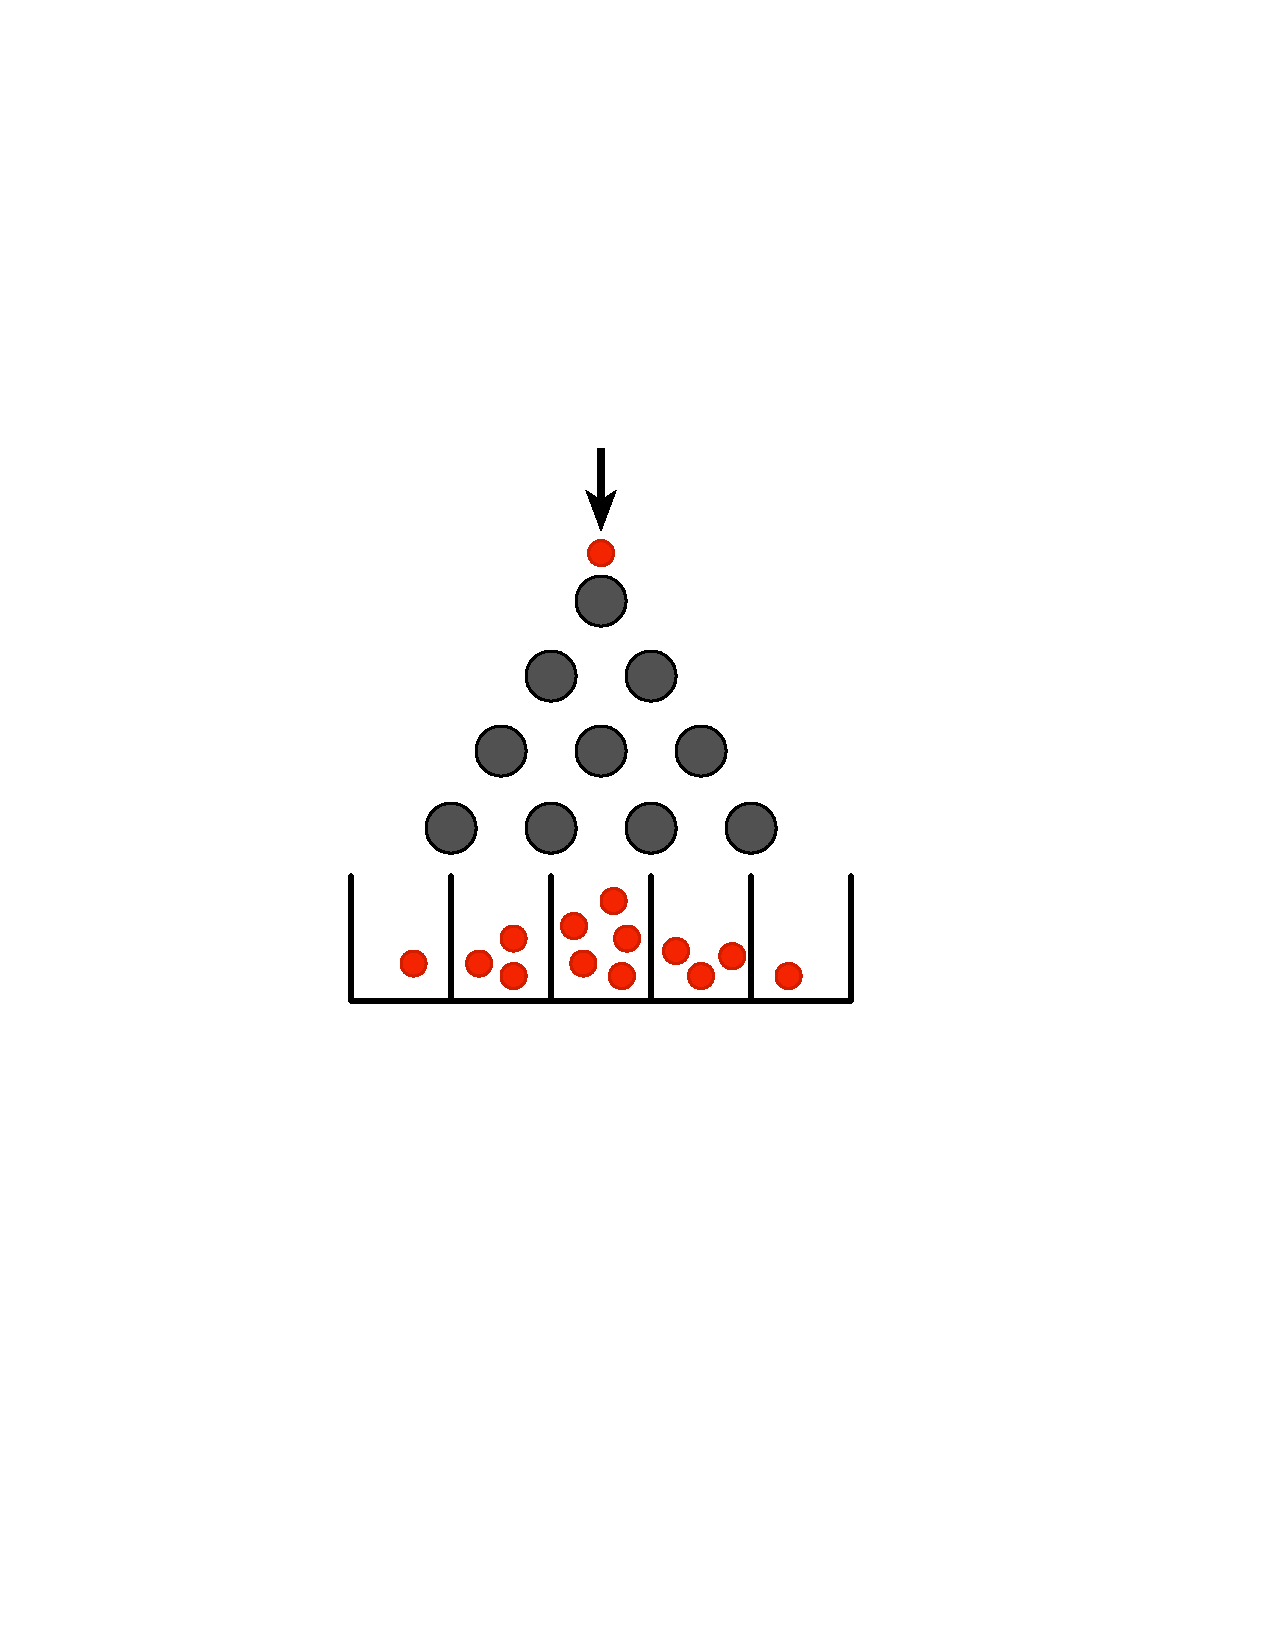
\includegraphics[width=0.3\textwidth]{galton_board}
\caption{The Galton board yields a very simple classical sampling problem. Balls (red) are input at the top and allowed to fall freely through the pyramid network of pegs (grey), at which balls bounce to the left or right with 50\% probability. At the output the balls are collected into buckets, which populate according to a binomial distribution\index{Binomial distribution}. The computational problem is to produce statistically accurate samples from such a device, which classically is efficiently implemented by sampling the binomial distribution.}	\label{fig:galton_board}\index{Galton board}
\end{figure}
